%% USPSC-Introducao.tex

% ----------------------------------------------------------
% Introdução (exemplo de capítulo sem numeração, mas presente no Sumário)
% ----------------------------------------------------------
\chapter[Introduction]{Introduction}
\label{ch: Intro}

During the last decade, the world has seen an increase in participation of renewable sources in power generation, leaded mainly by wind and solar energy. These green technologies provide an alternative to sources based on fossil fuel, lowering pollution levels and reducing greenhouse gas emissions. On the other hand, the power output from these sources rely on weather conditions and cannot be fully controlled.

This increase is seen worldwide, as part of policies to reduce the human impact on climate and the environment. This `renewable wave' is leaded mainly by European countries, specially in the European Union (EU), United States (US) and China. In particular, EU has set in 2010 a strategy plan to reduce its greenhouse emissions by at least 20\% compared to 1990 levels and increase the share of renewable sources to at least 20\% by 2020 \cite{Europe2020}.

Brazil does not lag far behind EU regarding renewable sources policies. In 2002, the country passed a bill that, among other actions, creates the Program of Incentive to Alternative Electric Energy Sources (PROINFA). This program aims to increase the share of wind, solar, small hydro and biomass energy production. The final goal is to have these energy sources corresponding to 10\% of Brazil's annual energy consumption by 2024 \cite{Brazil2002}.

\section{Wind Energy}

Those policies promoted the increase of wind energy participation, reaching a scenario where it is one of the main energy sources of some countries, such as Denmark and Ireland. In the EU, wind energy alone generated 362 TWh in 2018, covering 14\% of the electricity demand, a share 2\% higher than 2017, with wind turbines installed both onshore (within the countries) and offshore (in the ocean). Among the EU countries, Denmark leads in this sector, with 41\% of its demand supplied by wind power plants, followed by Ireland (28\%), Portugal (24\%) and Germany (21\%). The total installed capacity across the 28 EU countries is 178.8 GW, with Germany in first position, with a total installed capacity of 59.3 GW, followed by Spain and the United Kingdom (UK), with 23.5 and 21.0 GW installed, respectively \cite{WindEurope2019}. Figure \ref{fig: EUrank} displays the detailed percentage of electricity demand covered by wind in the EU.

\begin{figure}[h]
	\caption{Share of electricity demand in the EU covered by wind energy during 2018}
	\begin{center}
		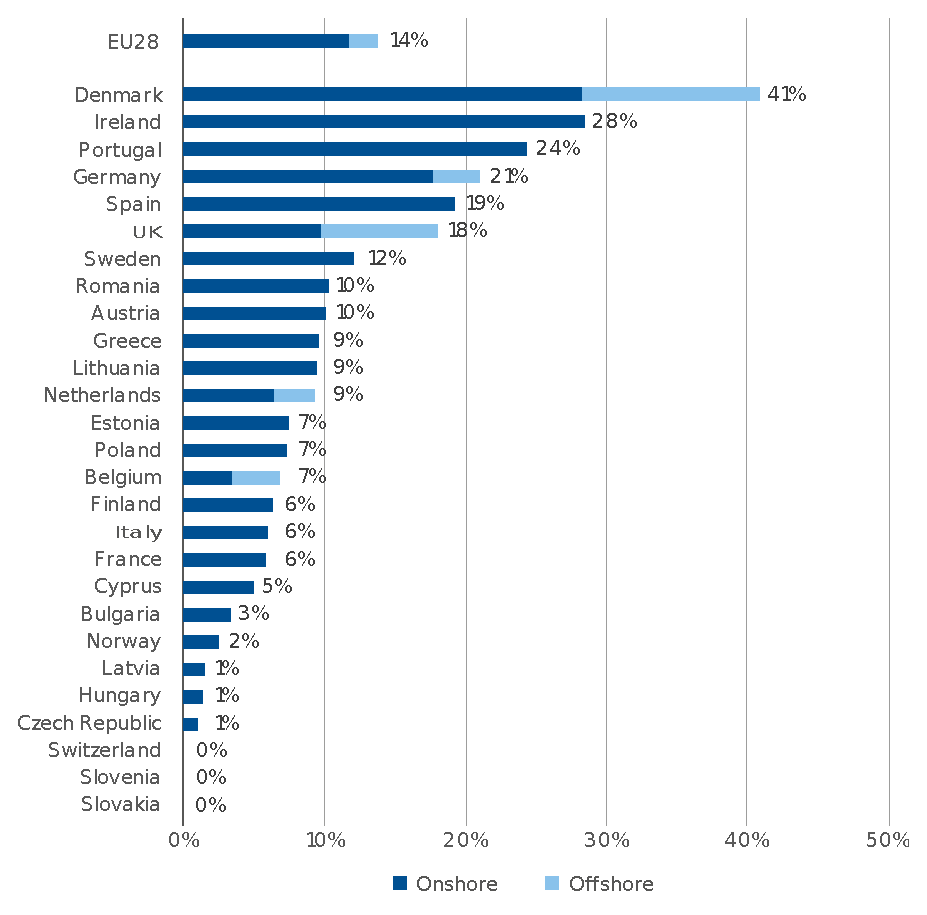
\includegraphics[scale=0.65]{Images/EUrank.eps}
	\end{center}
	\label{fig: EUrank}
	\legend{Source: Wind Europe, 2019}
\end{figure}

In Brazil, wind energy contributed to the electricity matrix with 42.4 TWh during 2017, resulting in a participation share of 7.2\%. For comparison, Itaipu, the largest power plant in Brazil, has produced 96.4 TWh during the same period. But, while other sources, such as hydro and coal, had its share lowered, wind energy had the highest increase among sources comparing to 2016, increasing its contribution by 26.5\% \cite{EPE2018}. 

Regarding the installed capacity, wind power plants appear in \nth{2} place, with 14.7 GW installed, only behind hydro power plants \cite{ABEEolica2018}, as shown in Figure \ref{fig: BRshare}. However, there is still plenty of energy yield for this source to be explored. In \cite{Atlas2001} is shown that Brazil has potential to generate 272.2 TWh per year, with an installed capacity of 143.5 GW. The Northeast Region has the higher potential, with an annual energy yield of 144.3 TWh and potential to host up to 75.0 GW . Also, the wind regime in the Northeast Region is complimentary to the water regime of the main river responsible to power generation in the region, as presented by Figure \ref{fig: WindWater}. This characteristic would help controlling reservoir water level during dry season, an important resource not only for power generation, but also irrigation of crops and water supply \cite{ANEEL2005}.

\begin{figure}[ht]
	\caption{Electricity generation in Brazil by source}
	\begin{center}
		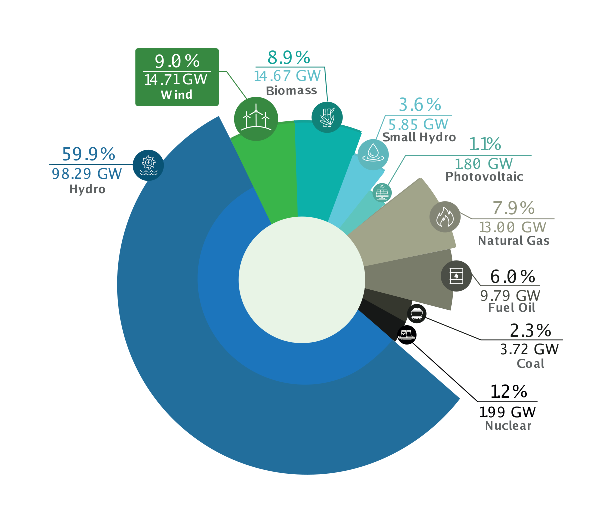
\includegraphics[scale=0.8]{Images/BRshare19.eps}
	\end{center}
	\label{fig: BRshare}
	\legend{Source: ABEE\'olica, 2018}
\end{figure}

\begin{figure}[hb]
	\caption{Wind and water regime in the Brazilian Northeast Region}
	\begin{center}
		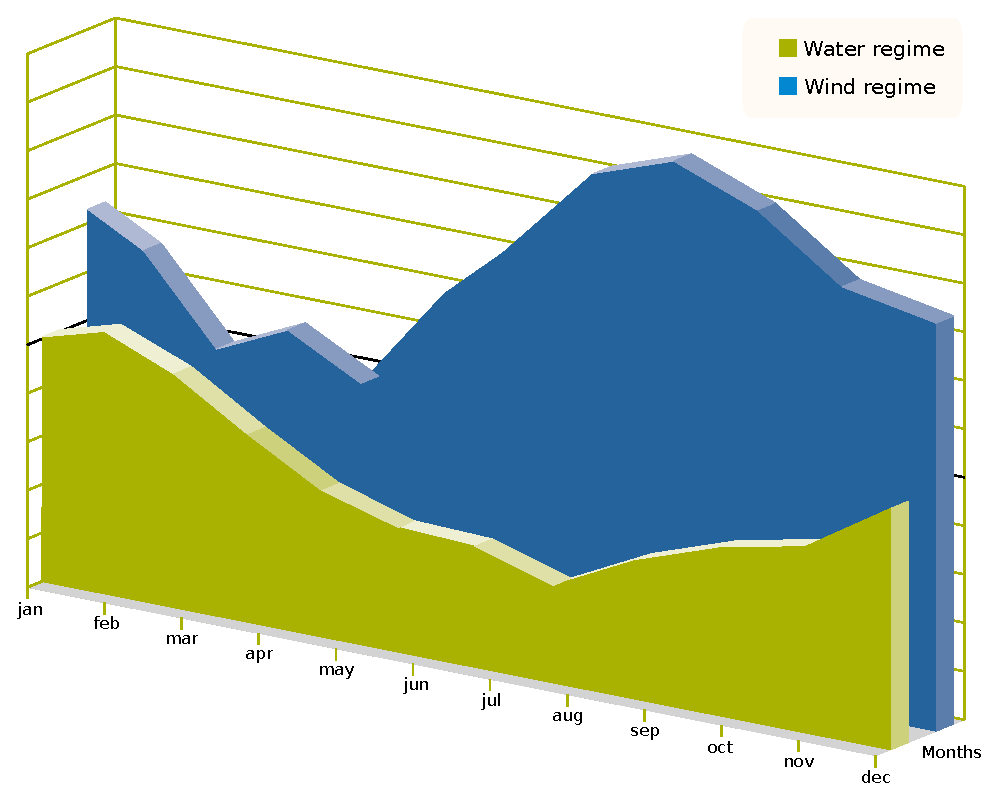
\includegraphics[scale=0.5]{Images/WindWater.eps}
	\end{center}
	\label{fig: WindWater}
	\legend{Source: ANEEL, 2005}
\end{figure}

Therefore, it is expected that wind energy will increase its participation in electricity generation in the next years. However, some aspects of the wind energy must be considered prior to the implementation on large scale of wind power plants.

The main difficulties are due to the nature of the energy source and the generator's characteristics. The wind regime is not constant and evenly distributed across the country, depending on the region's geography and vegetation. This results in a energy source that is not entirely reliable and concentrated on a certain area. Wind turbine generators usually have their rotor decoupled from the grid via frequency converter, leading to their low inertia. Thus, the system may experience stability problems during transients due to the high penetration of these machines \cite{Xiong2019}.

In order to maintain the electrical power system reliable, studies simulating various conditions must be performed beforehand, so the operators can be prepared for every occasion. These studies require mathematical models capable of adequately simulate the behaviour of every component on the grid.

\section{Difficulties in Representing Wind Power Plants}

With a growing share of energy covered by wind, system operators must consider how wind turbines affect the system stability during faults and maneuvers. To reach this goal, mathematical models capable of describing the behaviour of these machines are crucial. 

Obtaining these models, on the other hand, is not an easy task, considering the great amount of wind turbines available, with different manufacturers, technologies, sizes and characteristics. Thus, a model that describes well a particular power plant will not necessarily work for others. Also, due to confidentiality, manufacturers provide little or no information about their wind turbine generators. 

Particularly for wind power plants, an equivalent model is needed, since these facilities are usually widely spread and contain generators from different sizes and manufacturers. Besides, the distance to the substation is not the same for every generator in a wind power plants, as depicted in Figure \ref{fig: WPP}. Hence, having one model for every wind turbine within a power plant would result in a mathematical problem with high complexity and computational cost \cite{Erlich2012}.

\begin{figure}[h]
	\caption{Example of Wind Power Plant}
	\begin{center}
		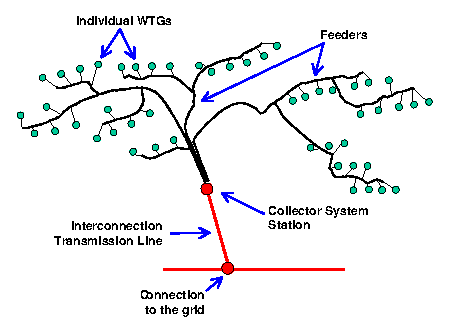
\includegraphics[scale=1.25]{Images/WPP.eps}
	\end{center}
	\label{fig: WPP}
	\legend{Source: Adapted from \cite{Muljadi2008}}
\end{figure}

\section{Research Goals}

The main goal of this research is to estimate parameters of an equivalent model of a wind power plant used in transient stability studies. To achieve this goal, a hybrid algorithm for parameter estimation will be developed combining two methods: Mean-Variance Mapping Optimization, an population-based heuristic approach, and Trajectory Sensitivity Method, a nonlinear approach. Also, as a secondary goal, a software, with graphical interface, for parameter estimation of nonlinear models will be developed. This research is a ongoing work of \cite{Cari2015}, that focused on the parameter estimation using only Trajectory Sensitivity Method.

\section{Work Organization}

This section summarizes how the remainder of the text is organized. Chapter \ref{ch: Mod} will focus on the generic models for wind turbine generators and power plants and the selected mathematical model for parameter estimation purposes will be presented. The hybrid estimation process proposed and its methods will be subject to chapter \ref{ch: Estim}, followed by the concept of the software under development on chapter \ref{ch: software}. On chapter \ref{ch: Res}, the partial results obtained and the ongoing progress will be discussed.